%


%-------------------------------'
%---------section  ---------------'
%-------------------------------'
\section{Independence for classes of events}
%-------------------------------'
%---------section  ---------------'
%-------------------------------'


\begin{definition}[{\bf Probability space}]
If $\Omega$ is a sample space, $\mathcal F$ is a $\sigma$-field on $\Omega$ and $P$ is a probability measure on $\mathcal F$, the triple $(\Omega, \mathcal F, P)$ is called a {probability space}.
\end{definition}

\begin{sectionassumption}
Throughout this section let $(\Omega, \mathcal F, P)$ denote a probability space and $\mathcal K$ be an arbitrary index set.
\end{sectionassumption}

\begin{definition}[{\bf Independent events}]
%Let $(\Omega, \mathcal F, P)$ be a probability space and $\mathcal K$ be an arbritary index set.
A collection of $\mathcal F$-sets $\{ A_k \}_{k\in\mathcal K}$ are said to be {independent} if for every finite index set $\mathcal H\subset \mathcal K$ the following identity holds:
\[ P\Bigl(\bigcap_{h\in\mathcal H}A_h\Bigr) = \prod_{h\in\mathcal H} P(A_h).\]
\end{definition}


\begin{definition}[{\bf Independent classes}]
%Let $(\Omega, \mathcal F, P)$ be a probability space and $\mathcal K$ be an arbritary index set.
Let $\mathscr A_k$ be a collection of $\mathcal F$-sets for each $k\in\mathcal K$ (i.e.\! $\mathscr A_k\subset \mathcal F$). Then  $\{ \mathscr A_k\}_{k\in \mathcal K} $ are  {independent classes} if for each choice $A_k\in\mathscr A_k$ the events $\{A_k\}_{k\in\mathcal K}$ are independent.
\end{definition}

\begin{theorem}{$\phantom{asfd}$}
%Let $(\Omega, \mathcal F, P)$ be a probability space and $\mathcal K$ be an arbritary index set. Then
\begin{enumerate}
\item {\bf (Subclasses).} If $\mathscr A_k\subset \mathscr B_k\subset \mathcal F$ for all $k\in\mathcal K$ and $\{\mathscr B_k\}_{k\in\mathcal K}$ are independent classes then  $\{\mathscr A_k\}_{k\in\mathcal K}$ are independent classes.
\item   {\bf (Augmentation).} $\bigl\{\mathscr A_k\bigr\}_{k\in\mathcal K}$ are independent classes if and only if  $\bigl\{\mathscr A_k\cup \{ \Omega \}\bigr\}_{k\in\mathcal K}$ are independent classes.
\item  {\bf (Simplified product). } If $\mathscr A_1,\ldots, \mathscr A_n$ are collections of $\mathcal F$-sets and $\Omega\in\mathscr A_k$ for each $k$, then $\mathscr A_1,\ldots, \mathscr A_n$ are independent classes if and only if
\[ P\Bigl(\bigcap_{k=1}^nA_k\Bigr) = \prod_{k=1}^n P(A_k).\]
for each choice $A_k\in\mathscr A_k$.
\end{enumerate}
\end{theorem}

\begin{theorem}[{\bf $\pi$-generators are enough}]
Suppose $\{\mathscr A_k\}_{k\in\mathcal K}$ are independent classes of  $\mathcal F$-sets such that each $\mathscr A_k$ is also a $\pi$-system. Then $\{\sigma\langle \mathscr A_k\rangle \}_{k\in\mathcal K}$ are independent classes.
\end{theorem}

\begin{theorem}[{\bf ANOVA}] Let $\mathscr A_1, \mathscr A_2,\ldots$ and $\mathscr B_1, \mathscr B_2,\ldots$ be classes of $\mathcal F$-sets which are $\pi$-systems. Then $\mathscr A_1, \mathscr A_2,\ldots,\mathscr B_1, \mathscr B_2,\ldots$ are all independent  if and only if the following three statements hold:
\begin{enumerate}
\item $\mathscr A_1, \mathscr A_2,\ldots$ are independent;
\item $\mathscr B_1, \mathscr B_2,\ldots$ are independent;
\item $\sigma\langle \mathscr A_1, \mathscr A_2,\ldots \rangle $ is independent of  $\sigma\langle \mathscr
B_1, \mathscr B_2,\ldots \rangle $.
\end{enumerate}
\end{theorem}


\begin{theorem}[{\bf ANOVA${}^*$}]
Consider the following array of $\pi$-systems of $\mathcal F$-sets
\[
\begin{array}{ccc}
\mathscr A_{1,1} & \mathscr A_{1,2} & \cdots \\
\mathscr A_{2,1} & \mathscr A_{2,2} & \cdots \\
\mathscr A_{3,1} & \mathscr A_{3,2} & \cdots \\
\vdots & \vdots & \ddots
\end{array}
\]
Each row may have a different number of columns (finite or infinite) and the number of rows may be finite or infinite.
Let $\mathscr R_1,\mathscr R_2,\ldots$ denote the $\sigma$-fields generated by the rows: $\mathscr R_i:=\sigma\langle \mathscr A_{i,1}, \mathscr A_{i,2} , \cdots \rangle $.
 Then the full collection  $\{ \mathscr A_{i,k} \}$ of $\pi$-systems are independent  if and only if the following two statements hold:
\begin{enumerate}
\item The $\pi$-systems within each row are independent;
\item The  $\sigma$-fields generated by the rows, $\mathscr R_1,\mathscr R_2,\ldots$, are independent.
\end{enumerate}
\end{theorem}



\begin{theorem}[{\bf Independent binary digits}]\label{ibd}
Let $H_n:=\{w\in(0,1]: d_n(w)=1  \}$ where $d_n$ denote the $n^\text{th}$ binary (nonterminating) digit from the basic spinner model in Section \ref{Bsec}. Then $H_1, H_2, \ldots$ are independent events under the model $P:\mathcal B_0^{(0,1]}\rightarrow [0,1]$ defined in Section \ref{Bsec}.
\end{theorem}



\subsection{Borel-Cantelli, Fatou and 0-1 laws}

\begin{definition}[{\bf Tail events}]
Let $\mathscr A_1, \mathscr A_2, \ldots$ be classes of $\mathcal F$-sets. Then
\[ \mathcal T :=\bigcap_{m=1}^\infty \sigma\langle \mathscr A_n: n\geq m\rangle \]
is called the {tail $\sigma$-field associated with $\mathscr A_1, \mathscr A_2, \ldots$}. Moreover, any event $T\in \mathcal T$ is called a {tail event}.
\end{definition}

\begin{theorem}[{\bf Kolmogorov's 0-1 Law}]
Suppose $\{\mathscr A_k\}_{k\in\mathcal K}$ are independent classes of  $\mathcal F$-sets such that each $\mathscr A_k$ is also a $\pi$-system. Then for any tail event $T\in\mathcal T$ either $P(T)=0$ or $P(T)=1$.
\end{theorem}

\begin{definition}[{\bf$\io$ and $\aall$}] Let $A_1, A_2, \ldots$ be subsets of $\Omega$. Then
\begin{align*}
\{A_n\, \io_n\} &:= \bigcap_{m=1}^\infty \bigcup_{n=m}^\infty A_n =: \limsup_{n\rightarrow \infty} A_n\\
\{A_n\, \aall_n \}&:= \bigcup_{m=1}^\infty \bigcap_{n=m}^\infty A_n =: \liminf_{n\rightarrow \infty} A_n
\end{align*}
\end{definition}

\begin{theorem}[{\bf $1^\text{st}$ Borel-Cantelli lemma}]
Let $A_1, A_2, \ldots$ be $\mathcal F$-sets. Then
\[ \sum_{n=1}^\infty P(A_n)<\infty \Longrightarrow P(A_n\, \io_n)=0. \]
\end{theorem}

\begin{theorem}[{\bf Fatou for sets}]
Let $A_1, A_2, \ldots$ be  $\mathcal F$-sets. Then
\begin{align*}
P(A_n\, \aall_n)&\leq \liminf_n P(A_n)\\
&\leq \limsup_n P(A_n)\leq P(A_n\, \io_n).
\end{align*}
\end{theorem}

\begin{theorem}[{\bf $2^\text{nd}$ Borel-Cantelli lemma}]
Let $A_1, A_2, \ldots$ be independent $\mathcal F$-sets. Then
\[ \sum_{n=1}^\infty P(A_n)=\infty \Longrightarrow P(A_n\, \io_n)=1. \]
\end{theorem}



\begin{exercise}
Let $\mathscr A_1,\ldots, \mathscr A_n$ be $\pi$-systems of $\mathcal F$-sets such that
\begin{equation}
\label{iee}
 P\Bigl( \bigcap_{k=1}^n A_k \Bigr) = \prod_{k=1}^n P(A_k)
\end{equation}
for each choice of $A_k\in\mathscr A_k$ for $k=1,\ldots, n$. (a) Show by simple example that the $\mathscr A_k$'s need not be independent. (b) Show that the $\mathscr A_k$'s will be independent if for each $k$, $\Omega$ is the countable union of $\mathscr A_k$-sets. Hint: for fixed $A_2,\ldots, A_n$ use the following general inclusion-exclusion formula to show that  (\ref{iee}) with $A_1$ replaced by any finite union of $\mathscr A_1$-sets. Here is the general inclusion-exclusion formula:
\[ P\Bigl( \bigcup_{i=1}^n B_i \Bigr)= \sum_{m=1}^n (-1)^{m-1}\sum_{i_1< i_2<\cdots<i_m} P(B_{i_1}\cap B_{i_2}\cap \cdots \cap B_{i_m}) \]
for any $\mathcal F$-sets $B_1, B_2,\ldots, B_n$.
\end{exercise}


\begin{exercise}
(a) For each $k=1,\ldots, n$ let $\mathcal P_k$ be a partition of $\Omega$ into countably many $\mathcal F$-sets. Show that the $\sigma$-fields $\sigma\langle\mathcal P_1\rangle,\ldots, \sigma\langle \mathcal P_n\rangle$ are independent if and only if (\ref{iee}) holds for each choice of $A_k$ from $\mathcal P_k$ for $k=1,\ldots, n$. (b) Use part (a) to show that $\mathcal F$-sets $A_1, \ldots, A_n$ are independent if and only if
\[
 P\Bigl( \bigcap_{k=1}^n B_k \Bigr) = \prod_{k=1}^n P(B_k)
\]
for each choice of $B_k$ as $A_k$ or $A_k^c$ for $k=1,\ldots, n$. (c) Use part (b) to show that the events $H_1,\ldots, H_n$ in Theorem \ref{ibd} are independent.
\end{exercise}






\begin{exercise}
Let $A_1, A_2, \ldots$ be $\mathcal F$-sets. Show that $P(A_n\io_n)=1$ if and only if $\sum_{n=1}^\infty P(A_n|A)$ diverges for every $\mathcal F$-set $A$ of nonzero probability. Hint: show $P(A_n\io_n)<1\Longleftrightarrow \sum_{n=1}^\infty P(A_n|A)<\infty$ for some $\mathcal F$-set $A$ with $P(A)>0$.
\end{exercise}
\begin{exerciseproof}
($\Longrightarrow$)
Suppose $P(A_n\io_n)<1$. Therefore  $P(A_n^c \aall_n) = P(\bigcup_{m=1}^\infty \bigcap_{n=m}^\infty A_n^c )>0$. In particular, there exists an $m_0\geq 1$ such that $ P(\bigcap_{n=m_0}^\infty A_n^c ) > 0$ (to prove this by contradiction just use countable-sub-additivity).
Now set $A :=  \bigcap_{n=m_0}^\infty A_n^c $. Notice $P(A)>0$ and for all $k> m_0$
\[P(A_k\cap A) = P(A_k \cap \bigcap_{n=m_0}^\infty A_n^c ) = 0.  \]
Therefore $\sum_{k=1}^\infty P(A_k \cap A)<\infty$ for some $\mathcal F$-set $A$ with $P(A)>0$.


($\Longrightarrow$) Suppose  $\sum_{n=1}^\infty P(A_n|A)<\infty$ for some $\mathcal F$-set $A$ with $P(A)>0$.
Now
\begin{align*}
\sum_{n=1}^\infty P(A_n \cap A)<\infty
&\Longrightarrow P[A_n\cap A \io_n] =0\\
&\Longrightarrow P\Bigl[\textstyle\bigcap_{m=1}^\infty \textstyle\bigcap_{n=m}^\infty  A_n\cap A \Bigl] =0\\
&\Longrightarrow P\Bigl[ A\cap \textstyle\bigcap_{m=1}^\infty \textstyle\bigcap_{n=m}^\infty  A_n \Bigl] =0\\
&\Longrightarrow P\bigl[ A\cap \{A_n \io_n \} \bigl] =0.
\end{align*}
Now if $P[A_n \io_n]=1$ then $0=P[A \cap  \{A_n \io_n \}] = P[A]$ which contradicts our assumption on $P[A]$. Therefore $P[A_n \io_n]<1$.
\end{exerciseproof}


\begin{exercise}
Let $P$ and $Q$ be probability measures on a $\sigma$-field $\mathcal F$ of subsets of a sample space $\Omega$.
\begin{itemize}
\item
$P$ and $Q$ are said to be {\bf singular}, denoted $P\perp Q$, if and only if there exists a set $F\in\mathcal F$ such that
\[P(F^c)=0=Q(F).\]
\item
P is said to be {\bf absolutely continuous with respect to $Q$}, denoted $P \ll Q$, if and only if
\[\text{$P(F)=0$ for every $\mathcal F$-set $F$ for which $Q(F)=0$.}  \]
\end{itemize}
Show that
\[P\perp Q \Longleftrightarrow \left[\begin{array}{c}
\text{there exists $\mathcal F$-sets $F_1, F_2,\ldots$ such that}\\
\text{$P(F_n^c)\rightarrow 0$ and $Q(F_n)\rightarrow 0$ as $n\rightarrow \infty$}
\end{array} \right] \]
and
\[P\ll Q \Longleftrightarrow  \lim_{\delta\downarrow 0}\Bigl( \sup\{ P(F)\colon \text{$F\in \mathcal F$ with $Q(F)\leq \delta$} \}\Bigr)=0. \]
\end{exercise}
\begin{exerciseproof}
({\sl $P\perp Q \Longrightarrow $ there exists $\mathcal F$-sets...}) Trivial.


({\sl  there exists $\mathcal F$-sets... $\Longrightarrow P\perp Q  $}) Choose a subsequence $n_k$ such that
\begin{align*}
\textstyle\sum_k Q(F_{n_k}) &< \infty \\
\textstyle\sum_k P(F^c_{n_k}) &< \infty.
\end{align*}
Therefore by the first Borel-Cantelli lemmas we have
\begin{align*}
Q(F_{n_k} \io_k) & =  0 \\
P(F^c_{n_k}\io_k) & =  0.
\end{align*}
Now By Fatou's lemma
\[ P[\{F_{n_k}\io_k\}^c] = P[F^c_{n_k}\aall_k ] \leq P[F^c_{n_k}\io_k ] =0 \]
Therefore $F:=\{F_{n_k}\io_k\}$ gives the desired set to establish that $P\perp Q$.

({\sl $P\ll Q \Longrightarrow \lim_{\delta\downarrow 0}$...}) \textcolor{red}{The following is a bit longer than it needs to be. Just try reductio.}
We first notice that the supremum in $\sup\{ P(F)\colon \text{$F\in \mathcal F$ with $Q(F)\leq \delta$}\}$ is attained. To see why let $F_n\in \mathcal F$ such that $Q(F_n)\leq \delta$ and $P(F_n)\rightarrow \sup\{\ldots\}$. By Fatou's lemma
\[
Q[F_n \aall_n]\leq \limsup_n Q(F_n)\leq \delta
\]
Since  $\{F_n \aall_n\}\in \mathcal F$ we have that
\begin{equation}
\label{abs cont from blw, 1}
P[F_n \aall_n] \leq \sup\{ P(F)\colon \text{$F\in \mathcal F$ with $Q(F)\leq \delta$}\}
\end{equation}
Also notice
\[
P[F_n \aall_n] =  \lim_m P[\bigcap_{n=m}^\infty F_n]\geq \lim_m P[ F_m] =\sup\{\ldots\}
\]
then, when combined with (\ref{abs cont from blw, 1}) gives that the supremum in $\sup\{ P(F)\colon \text{$F\in \mathcal F$ with $Q(F)\leq \delta$}\}$ is attained. Now, for each $\delta> 0$ let $F_\delta$  be the $\mathcal F$-set
 which makes the supermum attained. If we let $\delta_n \downarrow 0$, since $Q(F_{\delta_n})\leq \delta_{n}$ we can find a further sub sequence such that $\sum_k Q[F_{\delta_{n_k}}]<\infty$ so that $Q[F_{\delta_{n_k}} \io_k]=0$. Therefore $P[F_{\delta_{n_k}} \io_k]=0$ by the assumption $P\ll Q$. From Fatou again we have
 \begin{align*}
 0 &\leq \liminf_k P[F_{\delta_{n_k}}]\leq \limsup_k P[F_{\delta_{n_k}}]\leq P[F_{\delta_{n_k}} \io_k]=0
 \end{align*}
Therefore
\[
\lim_k \sup\{ P(F)\colon \text{$F\in \mathcal F$ with $Q(F)\leq \delta_{n_k}$}\}  =0
\]
To finish just notice that $\sup\{ P(F)\colon \text{$F\in \mathcal F$ with $Q(F)\leq \delta$}\}$ is monotonically decreasing in $\delta$ (and therefore a limit exists and that limit must equal every sub-sequential limit, for which we have found one which is zero).



({\sl $ \lim_{\delta\downarrow 0}\ldots \Longrightarrow P\ll Q$}) This one should be pretty easy. In particular,  let $F_0$ be a $ \mathcal F$-set such that $Q(F_0)=0$. Then to show $P\ll Q$ we need to establish that $P[F_0]=0$. To see why notice that
\begin{align*}
P(F_0)
&\leq  \sup\{ P(F)\colon \underbrace{\text{$F\in \mathcal F$ with $Q(F)\leq \delta$}}_{\text{$F_0$ is one of these}} \}.
\end{align*}
Now take the limits of both sides with respect to $\delta\rightarrow 0$. The right hand side limits to zero, by assumption. Therefore $P(F_0) = 0 $.
\end{exerciseproof}





%-------------------------------'
%---------section  ---------------'
%-------------------------------'
\subsection{Application: law of the iterated logarithm for coin flips}
%-------------------------------'
%---------section  ---------------'
%-------------------------------'


\begin{sectionassumption}
Throughout this section let $P:\mathcal B^{(0,1]}\rightarrow [0,1]$ be the probability model developed in Section \ref{Bsec} (and extended from the Carath\'eodory) for a uniform random number in $w\in (0,1]$. Also let $s_n$ be defined as in Section \ref{Bsec}.
\end{sectionassumption}


To motivate the law of the iterated logarithm lets start by discussing the difference between the weak law and strong law of large numbers.
\begin{align*}
\text{{\bf Weak law}:   } &\quad \lim_{n\rightarrow \infty} P\Bigl(\bigl|\frac{s_n}{n}\bigr| < \epsilon \Bigr) = 1, \,\text{ for all $\epsilon>0$;}\\
\text{{\bf Strong law}:   } &\quad  P\Bigl(\lim_{n\rightarrow \infty} \frac{s_n}{n} = 0 \Bigr) = 1.
\end{align*}
In some sense the difference can be explained as follows. The weak law fixes each $n$ then analyzes the ensemble of $s_n(\omega)/n$
over $\omega\in (0,1]$. In particular, the weak law says that for large $n$ it becomes increasingly rare to find $\omega$'s which satisfy $|s_n(\omega)/n| \geq \epsilon$.  Conversely the strong law fixes each $\omega\in (0,1]$ and analyzes the ensemble of $s_n(\omega)/n$  over $n$. In particular for almost all $\omega$,  $s_n(\omega)/n\rightarrow 0$ as $n\rightarrow \infty$.

Now lets make a similar analogy with the central limit theorem and the law of the iterated logarithm. From the strong law we know that   ${s_n(\omega)}/{n}$ converges to $0$ for nearly every $\omega$. We can then ask: at what rate? In particular, can we find a smaller denominator than $n$, call it $\ell_n$, so that  ${s_n}/{\ell_n}$ doesn't converge to zero. An answer is given by the central limit theorem
\[
\text{{\bf CLT}:   } \quad \lim_{n\rightarrow \infty} P\Bigl(\frac{s_n}{\sqrt{n}} < x \Bigr) = \Phi(x)
\]
where $\Phi(x) = P(Z\leq x)$ and $Z$ is a standard normal random variable. Notice two things. First, this suggests that the  ${s_n(\omega)}/{\sqrt{n}}$ reaches up to $\infty $ and down to $-\infty$ for different values of $\omega$ and $n$.
In particular for every cut-off $M$, there exists $n$ large enough so that $P\Bigl({s_n}/{\sqrt{n}} \geq M \Bigr)\approx 1- \Phi(M)>0$ to arbitrary precision.
Also, the central limit theorem is similar to the weak law in that it fixes each $n$ then analyzes the ensemble of $s_n(\omega)/\sqrt{n}$
over $\omega\in (0,1]$. The question then becomes, can one find an analogous form of the strong law such that  for each fixed $\omega$  one analyzes the ensemble rate of $s_n(\omega)$ as $n\rightarrow \infty$. The law of the iterated logarithm gives the right rate
\[
\text{{\bf LIL}:   } \quad P\Bigl(  \displaystyle\limsup_{n\rightarrow\infty} \frac{s_n}{\sqrt{2n\log\log n}} =1\Bigr)=1.
\]

Another way to think about the rate $\sqrt{2n\log \log n}$ is the effect due to the correlation of between $s_n$ across different values of $n$. The expected maximum of $n$ independent standard Gaussian random variables behaves as $\sqrt{2\log n}$. That maximum occurs uniformly on $\{1,2,\ldots, n \}$ and is therefore is expected to occur at index $n/2$.
If  $s_n/\sqrt{n}$ was not correlated across $n$, the central limit theorem might suggest that the maximum of $s_k/\sqrt{k}$ over $k\in \{1,2\ldots, n \}$ behaves on the order of $\sqrt{2\log n}$. This loosely suggests the maximum of $s_k$ over $k\in \{1,2\ldots, n \}$  behaves on the order $\sqrt{ n\log n}$. Now, in some sense, the LIIL says that the  correlation across $n$ will dampen the maximum excursions to be at most $\sqrt{ n\log \log n}$.

%%%%%%%%%%%%%%%%%%%
\begin{lemma}[{\bf Half of large deviation result}]
\label{LIL: usefull lemma 1}
For all $n\in \Bbb N$ and $x>0$ one has
\[
P\bigl(s_n/\sqrt{n} \geq x\bigr)\leq \exp\Bigl( -\frac{x^2}{2} \Bigr)
\]
\end{lemma}
\begin{proof} This was established in exercise \ref{exp ineq for sn}.
\end{proof}

The other half of the large deviation result we need is Lemma \ref{LIL: usefull lemma 2}, below. Combined these two lemmas give us  good approximations to   $P\bigl(s_n/\sqrt{n} \geq x_n\bigr)$ for large-ish values of $x_n$: large compared to $0$ but still small compared to $\sqrt{n}$ (if $x_n$ was larger then $\sqrt{n}$ then $P(s_n/\sqrt{n} > x_n)=0$). This is the key for deriving the Law of the Iterated Logarithm.
Also note that Lemma \ref{LIL: usefull lemma 1} was proved as an exercise but it is typically established using Markov's inequality, the moment generating function and the fact that $\frac{e^x + e^{-x}}{2} \leq \exp\left({x^2/2}\right)$.


\begin{lemma}[{\bf Other half of large deviation result}]
\label{LIL: usefull lemma 2}
If the sequence $\{x_n\}_{n\in\Bbb N}$ satisfies $0\leq x_n \rightarrow \infty$ and $x_n/\sqrt{n}\rightarrow 0$ as $n\rightarrow \infty$ then
 \[ P\bigl(s_n/\sqrt{n} \geq x_n\bigr)\geq \exp\Bigl( -\frac{x_n^2}{2} (1+o(1))\Bigr).\]
\end{lemma}
\begin{proof}
The general idea is to use the fact that $s_n=2\bigl(\sum_{k=1}^n d_k\bigr) -n$ where $\sum_{k=1}^n d_k\sim \text{Bin}(n,1/2)$.
Therefore we can write $P(s_n\geq \sqrt{n} x_n)$ as a sum $\sum_{i\in \mathcal I_n}P(s_n = i)$ where $i$ is the set of integers greater than $\sqrt{n} x_n$ and less than or equal to $n$. In fact, since we are trying to construct a lower bound we are free to discard terms in  $\mathcal  I_n$ which will give
\begin{align*}
P(&s_n\geq \sqrt{n} x_n) \geq \sum_{i\in\mathcal I_n} P(s_n = i).
\end{align*}
The main problem is how to find  $\mathcal I_n$ so that the right hand side is $\exp\bigl( -\frac{x_n^2}{2} (1+o(1))\bigr)$.

Lets start by getting some idea of how many integers we should include in  $\mathcal I_n$ by analysing how $P(s_n = i)$ behaves when $i\approx \sqrt{n}x_n
$. To make things a bit more precise let $i_n$ be a sequence of integers depending on $n$ such that $i_n\rightarrow \infty$ but $i_n/n \rightarrow 0$.
\begin{align}
P(s_n = i_n)
&=P\Bigl(\sum_{k=1}^n d_k = (i_n +n)/2\Bigr)\nonumber\\
&=\begin{pmatrix} n \\ (i_n +n)/2 \end{pmatrix} \frac{1}{2^n},\,\,\text{ if $(i_n +n)/2$ is an integer }\nonumber\\
&=\frac{n!}{\frac{i_n +n}{2}! \frac{n -i_n}{2}! } \frac{1}{2^n}\nonumber\\
& = \frac{2}{\sqrt{2\pi n}} [1+o(1)] \exp\left( - \frac{(1+o(1)) i_n^2}{2n} \right)\label{isright}
\end{align}
To see why (\ref{isright}) is true notice that by Stirling's formula we have $n! = (1+o(1)) \sqrt{2\pi n} n^n e^{-n}$. Therefore
\begin{align*}
\frac{n!}{\frac{i_n +n}{2}! \frac{n -i_n}{2}! }  \frac{1}{2^n}
&= \frac{(1+o(1))}{(1+o(1))^2} \\
&\qquad\times \frac{\sqrt{2\pi n} }{\sqrt{2\pi (n+i_n)/2}\sqrt{2\pi (n-i_n)/2}  } \\
&\qquad\times\frac{n^n}{ (n+i_n)^{(n+i_n)/2}(n-i_n)^{(n-i_n)/2}} \\
&\qquad\times \frac{ e^{-n}}{ e^{-(n+i_n)/2} e^{-(n-i_n)/2}  } \\
&= \frac{(1+o(1))}{(1+o(1))^2} \\
&\qquad\times \underbrace{\frac{1 }{\sqrt{2\pi (n+i_n) (n-i_n)/(4n)}  }}_{=:I}\\
&\qquad\times\underbrace{\left(\frac{n}{n+i_n}\right)^{(n+i_n)/2}\left(\frac{n}{n-i_n}\right)^{(n-i_n)/2}}_{=:I\!I}
\end{align*}
Notice
\begin{align*}
I&=\frac{1 }{\sqrt{2\pi (n+i_n) (n-i_n)/(4n)}  }\\
 &= \frac{2}{\sqrt{2\pi n}}\times \frac{1}{\sqrt{ (n+i_n) (n-i_n)/(n^2)}}\\
&= \frac{2}{\sqrt{2\pi n}}\times \frac{1}{\sqrt{1   -(i_n/n)^2}}= \frac{2}{\sqrt{2\pi n}} (1+o(1)).
\end{align*}
Secondly notice that $(1+x)\log(1+x)= x +\frac{1}{2}x^2+O(x^3)$ as $x\rightarrow 0$. Therefore
\begin{align*}
\log I\!I&= -\frac{1}{2}\bigl[ (n+i_n)\log \bigl(1+\frac{i_n}{n}\bigr) +  (n-i_n)\log \bigl(1-\frac{i_n}{n}\bigr) \bigr] \\
&=-\frac{n}{2}\bigl[\frac{i_n}{n} +\frac{1}{2}\frac{i_n^2}{n^2} - \frac{i_n}{n} +\frac{1}{2}\frac{i_n^2}{n^2}+O({i^3_n}/{n}^3)  \bigr] \\
&=-\frac{n}{2}\bigl[  \frac{i_n^2}{n^2}  +O({i^3_n}/{n}^3)  \bigr] = -\frac{i_n^2}{2n}\bigl[ 1  +\underbrace{O({i_n}/{n}}_{o(1)})  \bigr].
\end{align*}
To finish notice that   $\frac{(1+o(1))^2}{(1+o(1))^2} = [1+o(1)]$ which implies (\ref{isright}).
%\begin{align*}
%P(w\in\Omega:s_n(w) = i_n)& = \frac{2}{\sqrt{2\pi n}} \exp\left( - \frac{(1+o(1)) i_n^2}{2n} \right)\\
%& = \frac{2}{\sqrt{2\pi n}} \exp\Bigl(-\frac{i_n^2}{2n} \underbrace{\left[-\frac{2n}{i_n^2}o(1)\right]}_{\shortstack{$= o(1)$, \text{since} \\\text{$\sqrt{n}/i_n = o(1)$ }}} - \frac{(1+o(1)) i_n^2}{2n} \Bigr)\\
%& = \frac{2}{\sqrt{2\pi n}} \exp\left( - \frac{(1+o(1)) i_n^2}{2n} \right)
%\end{align*}
%\textcolor{blue}{I still don't see why we need $\sqrt{n}/i_n = o(1)$ for this preliminary step. The results seem to go fine with the approximation $P(w\in\Omega:s_n(w) = i_n) = \frac{2}{\sqrt{2\pi n}}(1+o(1)) \exp\left( - \frac{(1+o(1)) i_n^2}{2n} \right)
%$ }


Now, looking at (\ref{isright}) it is clear that we want $\mathcal I_n$ to contain about $\sqrt{2\pi n}$ terms that are near $\sqrt{n} x_n$ (so that we can apply  (\ref{isright})). In particular $\mathcal I_n$ denote the set of indices between $\sqrt{n}x_n$ and $\sqrt{n}x_n + 2\sqrt{\pi n}$ which have the same parity at $n$ (i.e. that $(i_n + n)/2$ is an integer).  Also let $i_n$ be the maximum integer in $\mathcal I_n$, which implies $i_n = \sqrt{n}x_n + 2\sqrt{\pi n} + O(1)$. Now
\begin{align*}
P(&s_n\geq \sqrt{n} x_n)\\
&\geq \sum_{i\in\mathcal I_n} P(s_n = i)\\
&\geq [\# \mathcal I_n] P(s_n = i_n),\,\,\text{since $\begin{pmatrix} n \\ (i +n)/2 \end{pmatrix}\geq \begin{pmatrix} n \\ (i_n +n)/2 \end{pmatrix}$}\\
&= [\sqrt{\pi n}+ O(1)] P(s_n = i_n)\\
&\geq \sqrt{2}\exp\left( - \frac{(1+o(1)) i_n^2}{2n} \right),\quad\text{by (\ref{isright})}\\
&\geq \exp\left( - \frac{(1+o(1)) i_n^2}{2n} \right) \\
&= \exp\left( - \frac{(1+o(1))\bigl[\sqrt{n}x_n +2\sqrt{\pi n} + O(1) \bigr]^2}{2n}  \right) \\
&= \exp\left( - \frac{x_n^2}{2} (1+o(1)) \right),\quad\text{since $x_n\rightarrow \infty$}.
\end{align*}

% \begin{align*}
% P(&s_n\geq \sqrt{n} x_n)\\
% &\geq \sum_{i\in\mathcal I_n} P(s_n = i)\\
% &\geq \sum_{i\in\mathcal I_n} P(s_n = i_n),\\
% &\qquad\qquad\qquad\text{since $\begin{pmatrix} n \\ (i +n)/2 \end{pmatrix}\geq \begin{pmatrix} n \\ (i_n +n)/2 \end{pmatrix}$}\\
% &= [\sqrt{\pi n}+ O(1)]P(s_n = i_n)\\
% &=\underbrace{ [\sqrt{\pi n}+ O(1)][1+o(1)]\frac{2}{\sqrt{2\pi n}} }_{ = \sqrt 2 +o(1)} \exp\left( - \frac{(1+o(1)) i_n^2}{2n} \right),\\
% &\qquad\qquad\qquad \text{by (\ref{isright}) since $i_n/n= O(x_n/\sqrt{n}) \rightarrow 0$} \\
% %&= [\sqrt{\pi n}+ O(1)]\frac{2}{\sqrt{2\pi n}} \exp\left( - \frac{(1+o(1)) i_n^2}{2n} \right) \\
% &= \sqrt{2} \exp\left( - \frac{(1+o(1)) i_n^2}{2n} \right)\\
% &\qquad\qquad\quad + \underbrace{ o(1)\exp\left( - \frac{(1+o(1)) i_n^2}{2n} \right)}_\text{$=o(1)$ since $i_n/\sqrt{n}=O(x_n)\rightarrow \infty$  }\\
% &\geq \exp\left( - \frac{(1+o(1)) i_n^2}{2n} \right).
% \end{align*}


% To finish the proof simply notice that
% \begin{align*}
% - \frac{(1+o(1)) i_n^2}{2n} & = - \frac{(1+o(1)) \bigl[\sqrt{n}x_n +2\sqrt{\pi n} + O(1) \bigr]^2}{2n} \\
% & = - \frac{x_n^2}{2} (1+o(1)) \bigl[1 + 2\sqrt{\pi}/x_n + O(1/(x_n\sqrt{n}) \bigr]^2 \\
% & = - \frac{x_n^2}{2} (1+o(1)) ,\quad\text{since $x_n\rightarrow \infty$}.
% \end{align*}
% Therefore $P(s_n\geq \sqrt{n} x_n) \geq \exp\bigl[ - \frac{x_n^2}{2} (1+o(1))  \Bigr]$.
\end{proof}




\begin{lemma}[{\bf Maximal inequality}]
\label{LIL: usefull lemma 3}
For all $n\in\Bbb N$ and every nonnegative integer $c$
\[ P\bigl( \max_{1\leq j\leq n} s_j \geq c \bigr)\leq 2P(s_n\geq c).\]
\end{lemma}
\begin{proof}
First write
\begin{align*}
P\bigl( \max_{1\leq j\leq n} s_j \geq c \bigr)&= P\bigl( \max_{1\leq j\leq n} s_j \geq c,\, s_n \geq c \bigr) \\
&\qquad\qquad+ P\bigl( \max_{1\leq j\leq n} s_j \geq c,\, s_n < c  \bigr)\\
&= P\bigl( s_n \geq c \bigr) + P\bigl( \max_{1\leq j\leq n} s_j \geq c,\, s_n < c  \bigr).
\end{align*}
Therefore all that remains is to show $ P\bigl( \max_{1\leq j\leq n} s_j \geq c,\, s_n < c  \bigr)\leq  P\bigl( s_n \geq c \bigr)$.
Start by segmenting the event $\{\max_{1\leq j\leq n} s_j \geq c\}$ corresponding to the first indicie $j$ for which $s_j= c$ (this must occur when  $ \max_{1\leq j\leq n} s_j \geq c$ since $s_n$ goes up or down with jumps of size $1$ and $c$ is a nonnegative integer). In particular, write
\[ \{  \max_{1\leq j\leq n} s_j \geq c \} =\bigcup_{j=1}^n \underbrace{\{s_1<c, \, \ldots,\, s_{j-1}<c,\, s_j= c \}}_{=:F_j} \]
Now
\begin{align*}
\{ &\max_{1\leq j\leq n} s_j \geq c\}\cap\{s_n < c\}\\
&= \bigcup_{j=1}^n F_j\cap  \{s_n < c\}\\
&= \bigcup_{j=1}^n \underbrace{F_j\cap  \{s_n - s_j<0\},}_\text{disjoint since the $F_j$'s are}\text{ since $\omega\in F_j$ implies $s_j(\omega)=c$}.
\end{align*}
Now notice two things. First $P(s_n - s_j<0)=P(s_n - s_j>0) $ by symmetry. Secondly, since $\{s_n - s_j<0 \}\in \sigma\langle z_{j+1},\ldots, z_n\rangle$ and $F_j\in \sigma\langle z_1,\ldots, z_j\rangle$, the event $\{s_n - s_j<0 \}$ is independent of $F_j$ (by ANOVA).
Therefore
\begin{align*}
P\bigl( &\max_{1\leq j\leq n} s_j \geq c,\, s_n < c \bigr)\\
&= \sum_{j=1}^n P\bigl( F_j\cap  \{s_n - s_j<0\} \bigr)\\
& = \sum_{j=1}^n P\bigl( F_j\bigr)P\bigl( s_n - s_j<0 \bigr)\text{ by independence}\\
& = \sum_{j=1}^n P\bigl( F_j\bigr)P\bigl( s_n - s_j>0 \bigr)\text{ by symmetry}\\
& = \sum_{j=1}^n P\bigl( F_j \cap \{s_n - s_j>0\} \bigr)\text{ by independence again}\\
& = \sum_{j=1}^n P\bigl( F_j \cap \{s_n > c\} \bigr)\text{ since $\omega\in F_j$ implies $s_j(\omega)=c$}\\
&= P\bigl( \max_{1\leq j\leq n} s_j \geq c,\, s_n > c \bigr)\\
&\leq  P\bigl( s_n > c \bigr) \\
&\leq  P\bigl( s_n \geq c \bigr).
\end{align*}
Therefore $P\bigl( \max_{1\leq j\leq n} s_j \geq c \bigr)\leq 2 P\bigl( s_n \geq c \bigr)$.
\end{proof}



\begin{theorem}[{\bf Law of the iterated logarithm for coin flips}]$\phantom{asdf}$
\label{thm: Law of the iterated logarithm}
\begin{enumerate}
\item\label{LIIL} $P\Bigl[  \displaystyle\limsup_{n\rightarrow\infty} \frac{s_n}{\sqrt{2n\log\log n}} =1 \Bigr]=1$;
\item $P\Bigl[  \displaystyle\liminf_{n\rightarrow\infty}  \frac{s_n}{\sqrt{2n\log\log n}} =-1 \Bigr]=1$.
\end{enumerate}
\end{theorem}

\begin{proof}
To make the formulas more readable let $\ell_n:=\sqrt{2n\log\log n}$.
Notice first that
 \begin{align*}
 &\{ \limsup_n \frac{s_n}{\ell_n}=1  \}\\
 &\qquad=\bigcap_{\epsilon\in (0,1)\cap \Bbb Q} \{ {s_n/\ell_n}> (1-\epsilon) \io_n \}\cap \{ {s_n/\ell_n}< (1+\epsilon) \aall_n \}.
 \end{align*}
  This implies that  $\{\limsup_n (s_n/\ell_n)=1  \}$  and $ \{\liminf_n (s_n/\ell_n)=-1  \}$ are Borel measurable.
Secondly notice that  by  symmetry we have
\begin{align*}
P\bigl[  \displaystyle\limsup_{n\rightarrow\infty} & (s_n/\ell_n) =1 \bigr] \\
& = P\bigl[  \displaystyle\liminf_{n\rightarrow\infty} (-s_n/\ell_n)  = -1 \bigr] \\
& = P\bigl[  \displaystyle\liminf_{n\rightarrow\infty} (s_n/\ell_n)  = -1 \bigr].
\end{align*}
We can also simply our proof by using countable sub-additivity
\begin{align*}
P\bigl[ \bigl\{ \displaystyle\limsup_{n\rightarrow\infty}& (s_n/\ell_n) =1\bigr\}^c \bigr]  \\
& \leq \sum_{\epsilon\in (0,1)\cap \Bbb Q} P[\{ {s_n/\ell_n}\leq (1-\epsilon) \aall_n \}] \\
&\qquad + \sum_{\epsilon\in (0,1)\cap \Bbb Q} P[\{ {s_n/\ell_n}\geq (1+\epsilon) \io_n \}].
\end{align*}
Therefore the proof will follow by establishing Lemmas \ref{LIIL: io lemma 1}
 and \ref{LIIL: io lemma 2} which state that for all $\epsilon>0$
 \begin{align*}
P[ s_n/\ell_n \geq  (1+\epsilon) \io_n ] &= 0 \\
P[ s_n/\ell_n > (1-\epsilon) \io_n ] &= 1
\end{align*}

\end{proof}


 Theorem \ref{thm: Law of the iterated logarithm} is interesting for a number of reasons. First, it gives a very detailed analysis of the Central Limit Theorem. Second, it shows the power of the Borel-Cantelli lemmas. Third, it is one of those theorems in probability which is extremely hard to see in simulations: $\sqrt{2n\log\log n}$ grows to slow for modern computers to probe. The following simulation is an attempt at illustrating  Theorem \ref{thm: LII} but we still don't see the required fluctuation from $+1$ to $-1$.
\begin{figure}[h]
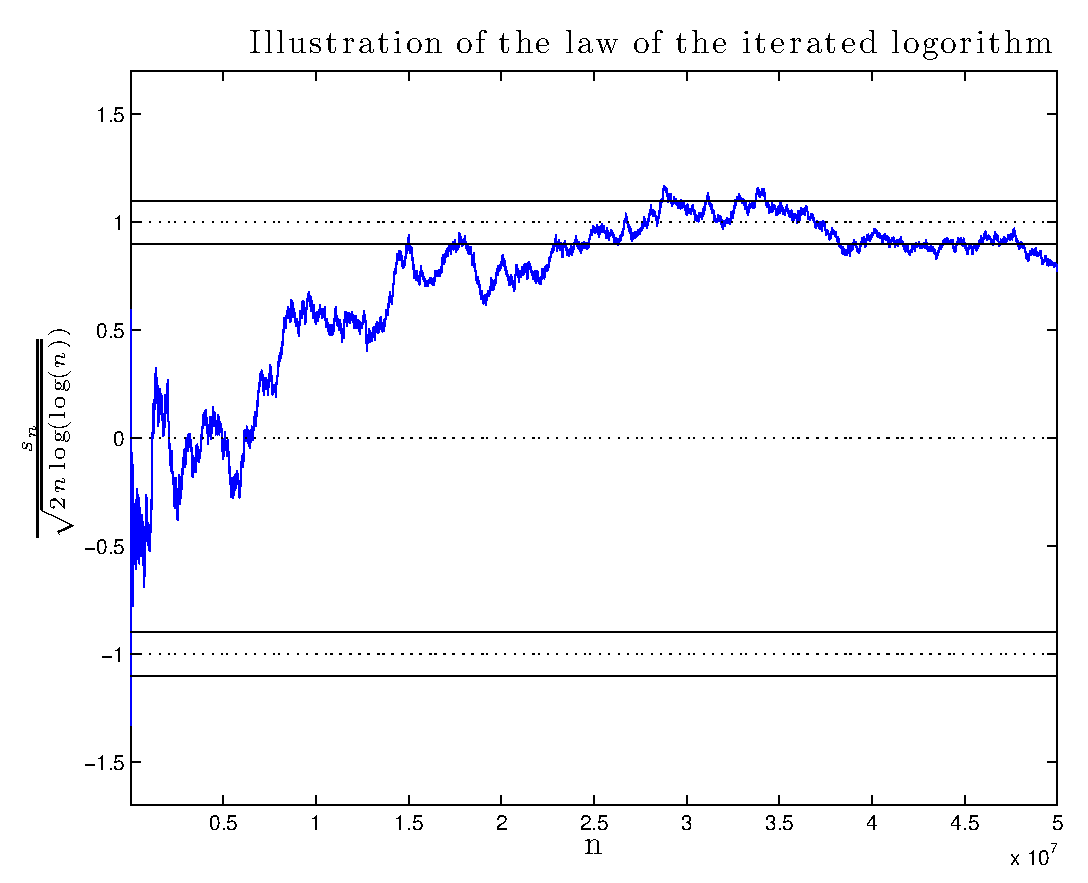
\includegraphics[height = 2.7in]{Measure/LIL.eps}
\end{figure}


\begin{lemma}
\label{LIIL: io lemma 1}
For all $\epsilon > 0 $
\begin{align*}
P[ s_n/\ell_n \geq  (1+\epsilon) \io_n ] = 0
\end{align*}
\end{lemma}
\begin{proof}
The obvious strategy is to use the first Borel-Cantelli lemma. In particular, it would be nice if we could show
\[
\sum_{n=1}^\infty P [ s_n/\ell_n \geq  (1+\epsilon)]<\infty
\]
which would give us the lemma. By the first half of the large deviation result we know $P [ s_n/\ell_n \geq  (1+\epsilon)]$ converge to zero as $n\rightarrow \infty$. Unfortunately, they do not converge fast enough for the first Borel-Cantelli. Taking a sub-sequence will get something summable but we would need to show that the events are well behaved between the sub-sequence. Fortunatly we can do this since the sets $\{s_n/\ell_n \geq  (1+\epsilon)\}$ overlap a lot. The strategy is to group the events $\{s_n/\ell_n \geq  (1+\epsilon)\}$ by unioning them into blocks, then apply Borel-Cantelli on the blocks. This will be sufficient since  the blocks occur infinity often if and only if the events $s_n/\ell_n \geq  (1+\epsilon)$ occur infinity often.  Controlling the probability of the blocks is done with the maximal inequality.

Let the $k^\text{th}$ block be defined
\[
B_k:= \bigcup_{j=n_{k-1}}^{n_k} \{ s_{j}/\ell_{j} \geq  (1+\epsilon) \}
\]
  where $n_k$ is  a (yet to be determined) subsequence. We  use maximal inequality  to bound $P[B_k]$ as follows
\begin{align*}
P[B_k]  &\leq P[\max_{n_{k-1}\leq j\leq n_k} s_j \geq (1+\epsilon)\min_{n_{k-1}\leq j\leq n_k} \ell_{j}] \\
 &\leq P[\max_{n_{k-1}\leq j\leq n_k} s_j \geq (1+\epsilon) \ell_{n_{k-1}}] \\
 &\leq P[\max_{j\leq n_k} s_j \geq (1+\epsilon) \ell_{n_{k-1}}] \\
 &\leq P[\max_{j\leq n_k} s_j \geq \lceil(1+\epsilon) \ell_{n_{k-1}}\rceil],\quad\text{since $s_j\in\Bbb Z$} \\
 &\leq 2P[ s_{n_k} \geq \lceil(1+\epsilon) \ell_{n_{k-1}}\rceil],\quad\text{maximal ineq} \\
 &\leq 2P[ s_{n_k} \geq (1+\epsilon) \ell_{n_{k-1}}] \\
 &\leq \exp\bigl( - \textstyle\frac{1}{2}(1+\epsilon)^2 \ell^2_{n_{k-1}}/n_{k} \bigr),\quad\text{half of large deviation}\\
 &\leq \exp\bigl( - (1+\epsilon)^2 n_{k-1}\log\log n_{k-1}/n_{k} \bigr)\\
 & = \left(\frac{1}{\log n_{k-1}} \right)^{ (1+\epsilon)^2\frac{n_{k-1}}{n_{k}} }.
\end{align*}
Now we just find $n_k$ which makes the last term summable over $k$. If $n_k\approx \theta^k$ one gets
\begin{align*}
\left(\frac{1}{\log n_{k-1}} \right)^{ (1+\epsilon)^2\frac{n_{k-1}}{n_{k}} }
& \approx  \left(\frac{1}{(k-1)\log\theta} \right)^{ (1+\epsilon)^2\frac{1}{\theta} }
\end{align*}
which is summable if $(1+\epsilon)^2\frac{1}{\theta} >1$. We also need that   $\theta > 1$  since we need $n_k\rightarrow \infty$ as $k\rightarrow \infty$. Luckily there does exist such a $\theta$ for which $(1+\epsilon)^2> \theta > 1$.
\end{proof}

\begin{lemma}
\label{LIIL: io lemma 2}
For all $\epsilon >0 $
\begin{align*}
P[ s_n/\ell_n > (1-\epsilon) \io_n ] = 1
\end{align*}
\end{lemma}
\begin{proof}
In the previous lemma we presented a technique to adjust the first Borel-Cantelli lemma in the case the summability condition doesn't hold. For this  lemma we want to use the second Borel-Cantelli lemma but, again, it doesn't directly apply since the condition that the events $s_n/\ell_n > (1-\epsilon)$ are independent does not hold. Here is a generic technique to get around this obstacle. Find subsequence $n_k$ and subsets
\[
I_k \subset   \{s_{n_k}/\ell_{n_k} > (1-\epsilon)\}
\]
such that $I_k$'s  are independent and $\sum_k P[I_k]=\infty$ so that $P[I_k \io_k]=1$ (which would then give the lemma). Unfortunately, even this doesn't work. What ends up working is to find two sets $A_k$ $I_k$ such that
\begin{align}
&A_k\cap I_k \subset \{s_{n_k}/\ell_{n_k} > (1-\epsilon)\}  \label{ABns in wwt}\\
&\text{$I_k$ are independent and $\textstyle\sum_k P[I_k]=\infty$} \label{Bns ind}\\
&\text{$A_k$ are not independent but $P[A_k \aall_k] = 1$.}\label{Ans Borel}
\end{align}
To see why this is sufficient notice that (\ref{Bns ind}) implies $P[I_k \io_k] = 1$ by the second Borel-Cantelli lemma. Then
\begin{align*}
&\text{ $P[A_k \aall_k] = 1$ and $P[I_k \io_k]=1$ } \\
&\qquad\Longrightarrow P[A_k \cap I_k \io_k] = 1 \\
&\qquad\overset{(\ref{ABns in wwt})}\Longrightarrow  P[s_{n_k}/\ell_{n_k} > (1-\epsilon) \io_k] = 1
\end{align*}
Therefore (\ref{ABns in wwt}), (\ref{Bns ind}) and (\ref{Ans Borel}) are sufficient to establish the lemma.

Figuring out how to define $I_k$ and $A_k$ are the tricky parts. The intuition is that if your going to get independent events you need to look at increments of $s_{n}$. Define
\begin{align*}
I_k &:= \{s_{n_k}-s_{n_{k-1}} \geq (1-\epsilon/2)\ell_{n_k}  \} \\
A_k &:= \{ s_{n_{k-1}} > -(\epsilon/2)\ell_{n_k}  \}.
\end{align*}
Clearly  $I_k \cap A_k \subset \{s_{n_k}/\ell_{n_k} > (1-\epsilon)\}$ so that (\ref{ABns in wwt}) holds. Moreover, the $I_k$'s  are independent.
To show (\ref{Ans Borel})
\begin{align*}
P[A_k \aall_k] &= P\Bigl[s_{n_{k-1}} > -(\epsilon/2)\ell_{n_k} \aall_k\Bigr] \\
 &= P\Bigl[s_{n_{k-1}} < (\epsilon/2)\ell_{n_k} \aall_k\Bigr],\quad\text{by symmetry} \\
&= P\Bigl[\frac{s_{n_{k-1}}}{\ell_{n_{k-1}}} < (\epsilon/2)\frac{ \ell_{n_k} }{ \ell_{n_{k-1}} } \aall_k\Bigr] \\
&= 1- P\Bigl[\frac{s_{n_{k-1}}}{\ell_{n_{k-1}}} \geq (\epsilon/2)\frac{ \ell_{n_k} }{ \ell_{n_{k-1}} } \io_k\Bigr] \\
&= 1,\,\text{by Lemma \ref{LIIL: io lemma 1} if \textcolor{blue}{$\frac{\ell_{n_k}}{\ell_{n_{k-1}}}\rightarrow \infty$.}}
\end{align*}
To show (\ref{Bns ind}) notice
\begin{align}
P[I_k] &= P\Bigl[ s_{n_k}-s_{n_{k-1}}\geq(1-\epsilon/2)\ell_{n_k}\Bigr] \nonumber\\
&= P\Bigl[s_{n_k-n_{k-1}}\geq(1-\epsilon/2)\ell_{n_k}\Bigr] \nonumber\\
&\geq P\Bigl[\frac{s_{n_k-n_{k-1}}}{\sqrt{n_k - n_{k-1}}}  \geq \frac{(1-\epsilon/2)\ell_{n_k}}{\sqrt{n_k - n_{k-1}}} \Bigr] \nonumber\\
&\geq \exp\Bigl(-\frac{1}{2}\Bigl[\frac{(1-\epsilon/2)\ell_{n_k}}{\sqrt{n_k - n_{k-1}}}\Bigr]^2(1+o(1))  \Bigr),\label{make this diverge}\\
&\qquad\qquad\text{\textcolor{blue}{by Lemma \ref{LIL: usefull lemma 2} if:}}\nonumber\\
&\qquad\qquad\quad\text{ \textcolor{blue}{$\textstyle\frac{\ell_{n_k}}{\sqrt{n_k - n_{k-1}}}\rightarrow \infty$ and  }}\nonumber\\
&\qquad\qquad\quad\text{ \textcolor{blue}{$\textstyle\frac{1}{\sqrt{n_k - n_{k-1}}}\frac{\ell_{n_k}}{\sqrt{n_k - n_{k-1}}}\rightarrow 0$ and }}\nonumber\\
&\qquad\qquad\quad\text{ \textcolor{blue}{$n_k - n_{k-1}\rightarrow \infty$. }}\nonumber
\end{align}
To finish the proof of (\ref{Ans Borel}) and (\ref{Bns ind}) we need to find $n_k\rightarrow \infty$ such that $\ell_{n_k}$ satisfies the above conditions and the \textcolor{blue}{sum of (\ref{make this diverge}) diverges}.

A subsequence of the form $n_k := \lfloor\exp(k^\theta)\rfloor$ will work. To check the conditions notice

\begin{align*}
\frac{\ell_{n_k}}{\ell_{n_{k-1}}}
& \sim \frac{ \sqrt{2 \exp(k^\theta) \log k^\theta} }{\sqrt{2 \exp((k-1)^\theta) \log (k-1)^\theta}} \\
& =  \exp\Bigl(\frac{k^\theta - (k-1)^\theta}{2}\Bigr) \frac{\log k}{\log (k-1)}  \\
& =  \exp\Bigl(\frac{\theta(k^*)^{\theta-1}}{2}\Bigr) (1 + o(1)),\quad\text{where $k-1\leq k^*\leq k$} \\
& \longrightarrow  \infty, \quad\text{\textcolor{red}{if  $\theta > 1$}.}
\end{align*}
Also
\begin{align*}
n_k - n_{k-1} & \sim  \exp(k^\theta) - \exp((k-1)^\theta) \\
&= \theta (k^*)^{(\theta-1)} \exp((k^*)^\theta) ,\quad\text{where $k-1\leq k^*\leq k$} \\
&\longrightarrow \infty,\quad\text{\textcolor{red}{if $\theta > 0 $.}}
\end{align*}
And therefore
\begin{align*}
\frac{\ell_{n_k}}{\sqrt{n_k - n_{k-1}}}
& \sim \frac{\sqrt{2 \exp(k^\theta) \log k^\theta}}{\sqrt{ \exp(k^\theta) - \exp((k-1)^\theta) }}   \\
&  = \frac{\sqrt{2\theta\log k}}{\sqrt{ 1 - \exp((k-1)^\theta-k^\theta)  }}  \\
& = \frac{\sqrt{2\theta\log k}}{\sqrt{ 1 - o(1)  }}\\
& \longrightarrow \infty.
\end{align*}
Clearly we now have that  $\frac{\ell_{n_k}}{{n_k - n_{k-1}}}  \longrightarrow 0.$
Finally we need to show that the sum of (\ref{make this diverge}) over $k$ diverges.  The individual terms are
\begin{align*}
\exp\Bigl(-\frac{1}{2}\Bigl[&\frac{(1-\epsilon/2)\ell_{n_k}}{\sqrt{n_k - n_{k-1}}}\Bigr]^2(1+o(1))  \Bigr) \\
& \sim \exp\Bigl(-\frac{(1-\epsilon/2)^2}{2}2\theta \log k   \Bigr) \\
& = \exp\Bigl(-{(1-\epsilon/2)^2}\theta \log k   \Bigr) \\
& = k ^ {-{(1-\epsilon/2)^2}\theta}
\end{align*}
the sum of the above terms over $k$ diverges if $(1-\epsilon/2)^\theta  < 1$, i.e. \textcolor{red}{ if $\theta < \frac{1}{(1-\epsilon)^2}$}. Now putting all the  conditions on $\theta$ together says that we simply need to choose $\theta$ such that
\[ 1<\theta <\frac{1}{(1-\epsilon/2)^2} .\]
\end{proof}
